\documentclass[convert, tikz]{standalone}
%\usepackage{xcolor}
\begin{document}
%\pagecolor[RGB]{255,255,254}
  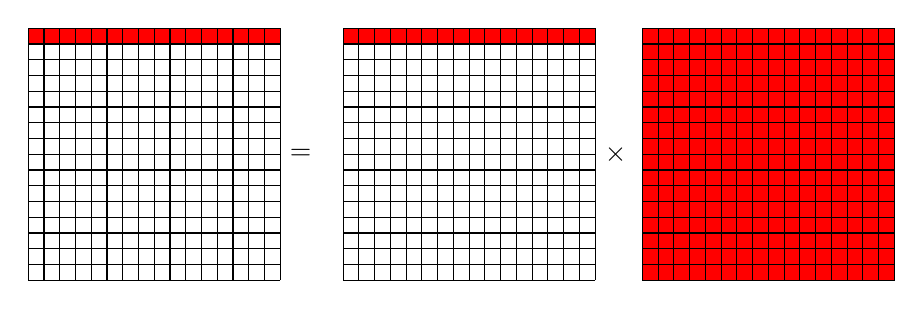
\begin{tikzpicture}[scale=0.2]
    \begin{scope}
      \draw[fill=red] (0,15)  rectangle (16,16);
      \draw[fill=red] (20,15) rectangle (36,16);
      \draw[fill=red] (39,0)  rectangle (55,16);
      \draw(0,0) grid(16,16);
      \draw(20,0) grid(36,16);
      \draw(39,0) grid(55,16);
      \node[right] at (16,8) {$=$};
      \node[right] at (36,8) {$\times$};
    \end{scope}
  \end{tikzpicture}
\end{document}
